%%**************************************************************
%% Vorlage fuer Bachelorarbeiten (o.ä.) der DHBW
%%
%% Autor: Tobias Dreher, Yves Fischer, Michael Gruben, Markus Barthel
%% Datum: 06.07.2011 - 22.08.2014
%%
%% Autor: Ferdinand König und Maximilian Köhler
%% Datum: 2020 - 2022
%%**************************************************************

%!TEX root = ../main.tex

%
% Nahezu alle Einstellungen koennen hier getaetigt werden
%

\RequirePackage[l2tabu, orthodox]{nag}	% weist in Commandozeile bzw. log auf veraltete LaTeX Syntax hin

\documentclass[%
    % final,
	pdftex,
	twoside,			% Einseitiger Druck (oneside) oder zweiseitig (twoside)
	headings=openright,	% Kapitelanfänge immer auf rechter Seite (bei zweiseitig)
	cleardoublepage=empty,	% Leere Vakatseiten
	12pt,				% Schriftgroesse
	parskip=half,		% Halbe Zeile Abstand zwischen Absätzen (half).
%	topmargin = 10pt,	% Abstand Seitenrand (Std:1in) zu Kopfzeile [laut log: unused]
	headheight = 20pt,	% Höhe der Kopfzeile
%	headsep = 30pt,	% Abstand zwischen Kopfzeile und Text Body  [laut log: unused]
	headsepline,		% Linie nach Kopfzeile.
	% footsepline,		% Linie vor Fusszeile.
	footheight = 10pt,	% Höhe der Fusszeile
	abstracton,		% Abstract Überschriften
	DIV=calc,		% Satzspiegel berechnen
	headinclude=false,	% Kopfzeile nicht in den Satzspiegel einbeziehen
	footinclude=false,	% Fußzeile nicht in den Satzspiegel einbeziehen
	listof=totoc,		% Abbildungs-/ Tabellenverzeichnis im Inhaltsverzeichnis darstellen
	toc=bibliography,	% Literaturverzeichnis im Inhaltsverzeichnis darstellen
	pointlessnumbers,
	fleqn,
	chapterprefix=true,
  appendixprefix=false,
	% bibliography=openstyle
]{scrreprt}	% Koma-Script report-Klasse (scrreprt), fuer laengere Bachelorarbeiten alternativ auch: scrbook

\raggedbottom

% Einstellungen laden
\usepackage{xstring}
\usepackage[utf8]{inputenc}
\usepackage[T1]{fontenc}

\newcommand{\einstellung}[1]{%
  \expandafter\newcommand\csname #1\endcsname{}
  \expandafter\newcommand\csname setze#1\endcsname[1]{\expandafter\renewcommand\csname#1\endcsname{##1}}
}
\newcommand{\langstr}[1]{\einstellung{lang#1}}

\einstellung{matrikelnr}
\einstellung{titel}
\einstellung{kurs}
\einstellung{datumAbgabe}
\einstellung{firma}
\einstellung{firmenort}
\einstellung{abgabeort}
\einstellung{abschluss}
\einstellung{studiengang}
\einstellung{dhbw}
\einstellung{betreuer}
\einstellung{gutachter}
\einstellung{zeitraum}
\einstellung{arbeit}
\einstellung{autor}
\einstellung{sprache}
\einstellung{schriftart}
\einstellung{seitenrand}
\einstellung{kapitelabstand}
\einstellung{spaltenabstand}
\einstellung{zeilenabstand}
\einstellung{zitierstil}
 % verfügbare Einstellungen
%%%%%%%%%%%%%%%%%%%%%%%%%%%%%%%%%%%%%%%%%%%%%%%%%%%%%%%%%%%%%%%%%%%%%%%%%%%%%%%
%                                   Einstellungen
%
% Hier können alle relevanten Einstellungen für diese Arbeit gesetzt werden.
% Dazu gehören Angaben u.a. über den Autor sowie Formatierungen.
%%%%%%%%%%%%%%%%%%%%%%%%%%%%%%%%%%%%%%%%%%%%%%%%%%%%%%%%%%%%%%%%%%%%%%%%%%%%%%%


%%%%%%%%%%%%%%%%%%%%%%%%%%%%%%%%%%%% Sprache %%%%%%%%%%%%%%%%%%%%%%%%%%%%%%%%%%%
%% Aktuell sind Deutsch und Englisch unterstützt.
%% Es werden nicht nur alle vom Dokument erzeugten Texte in
%% der entsprechenden Sprache angezeigt, sondern auch weitere
%% Aspekte angepasst, wie z.B. die Anführungszeichen und
%% Datumsformate.
\setzesprache{en} % de oder en
%%%%%%%%%%%%%%%%%%%%%%%%%%%%%%%%%%%%%%%%%%%%%%%%%%%%%%%%%%%%%%%%%%%%%%%%%%%%%%%%



%%%%%%%%%%%%%%%%%%%%%%%%%%%%%%%%%%% Angaben  %%%%%%%%%%%%%%%%%%%%%%%%%%%%%%%%%%%
%% Die meisten der folgenden Daten werden auf dem
%% Deckblatt angezeigt, einige auch im weiteren Verlauf
%% des Dokuments.
\setzematrikelnr{23176975}
\setzekurs{}
\setzetitel{Modeling of Fast-Switching Transformers\\for Voltage Stability Studies in Python}
\setzedatumAbgabe{May 2nd, 2025}
\setzefirma{}
\setzefirmenort{}
\setzeabgabeort{Erlangen}
\setzestudiengang{Energy Technology}
\setzebetreuer{Ilya Burlakin, M. Sc.}
\setzebetreuerzwei{Georg Kordowich, M. Sc.}
\setzegutachter{Univ.-Prof. Dr.-Ing. Matthias Luther\\Univ.-Prof. Dr.-Ing. Johann Jäger}
\setzezeitraum{02nd November 2024\ -\ 01st May 2025}
\setzearbeit{Master Thesis}
\setzeautor{Maximilian Markus Veit Köhler, B. Eng.}
\setzeversion{0.1}
\setzeoffset{0mm}
\setzebcor{0.7cm}
\setzecutoff{4cm}
\setzechapteroneoffset{4.5cm}

\newcommand{\prefacelogo}{
  \RaggedLeft
  \begin{minipage}[c]{4cm}
    \RaggedLeft
    \textit{The author was powered by}
  \end{minipage}
  \begin{minipage}[c]{4.5cm}
    \RaggedLeft
    
\includegraphics[width=4cm]{intro/crazy_sheep.png}
  \end{minipage}
}



%%%%%%%%%%%%%%%%%%%%%%%%%%%% Literaturverzeichnis %%%%%%%%%%%%%%%%%%%%%%%%%%%%%%
%% Bei Fehlern während der Verarbeitung bitte in ads/header.tex bei der
%% Einbindung des Pakets biblatex (ungefähr ab Zeile 110,
%% einmal für jede Sprache), biber in bibtex ändern.
\newcommand{\ladeliteratur}{%
\addbibresource{literatur.bib}
%\addbibresource{weitereDatei.bib}
}
%% Zitierstil
%% siehe: http://ctan.mirrorcatalogs.com/macros/latex/contrib/biblatex/doc/biblatex.pdf (3.3.1 Citation Styles)
%% mögliche Werte z.B numeric-comp, alphabetic, authoryear, numeric
\setzezitierstil{ieee}
%\setzezitierstil{alphabetic}
%\setzezitierstil{authoryear}




%%%%%%%%%%%%%%%%%%%%%%%%%%%%%%%%% Layout %%%%%%%%%%%%%%%%%%%%%%%%%%%%%%%%%%%%%%%
%% Verschiedene Schriftarten
% laut nag Warnung: palatino obsolete, use mathpazo, helvet (option scaled=.95), courier instead
\setzeschriftart{charter} % palatino oder goudysans, lmodern, libertine, mathptmx
% palatino oder lmodern ganz nett

%% Paket um Textteile drehen zu können
%\usepackage{rotating}
%% Paket um Seite im Querformat anzuzeigen
%\usepackage{lscape}

%% Seitenränder
% \setzeseitenrand{2.5cm}

%% Abstand vor Kapitelüberschriften zum oberen Seitenrand
\setzekapitelabstand{0pt}

%% Spaltenabstand
\setzespaltenabstand{10pt}
%%Zeilenabstand innerhalb einer Tabelle
\setzezeilenabstand{1.3}




%%%%%%%%%%%%%%%%%%%%%%%%%%%%% Verschiedenes  %%%%%%%%%%%%%%%%%%%%%%%%%%%%%%%%%%%
%% Farben (Angabe in HTML-Notation mit großen Buchstaben)
\newcommand{\ladefarben}{%
	\definecolor{LinkColor}{HTML}{00007A}
	% \definecolor{ListingBackground}{HTML}{FCF7DE}
}

%%Mathematikpakete benutzen (Pakete aktivieren)
\usepackage{amsmath}
\usepackage{amssymb}

%% Programmiersprachen Highlighting (Listings)
\newcommand{\listingsettings}{%
	\lstset{%
		language=Java,			% Standardsprache des Quellcodes
		numbers=left,			% Zeilennummern links
		stepnumber=1,			% Jede Zeile nummerieren.
		numbersep=5pt,			% 5pt Abstand zum Quellcode
		numberstyle=\tiny,		% Zeichengrösse 'tiny' für die Nummern.
		breaklines=true,		% Zeilen umbrechen wenn notwendig.
		breakautoindent=true,	% Nach dem Zeilenumbruch Zeile einrücken.
		postbreak=\space,		% Bei Leerzeichen umbrechen.
		tabsize=2,				% Tabulatorgrösse 2
		basicstyle=\ttfamily\footnotesize, % Nichtproportionale Schrift, klein für den Quellcode
		showspaces=false,		% Leerzeichen nicht anzeigen.
		showstringspaces=false,	% Leerzeichen auch in Strings ('') nicht anzeigen.
		extendedchars=true,		% Alle Zeichen vom Latin1 Zeichensatz anzeigen.
		captionpos=b,			% sets the caption-position to bottom
		% backgroundcolor=\color{ListingBackground}, % Hintergrundfarbe des Quellcodes setzen.
    backgroundcolor=\color{white!50},
		xleftmargin=0pt,		% Rand links
		xrightmargin=0pt,		% Rand rechts
		frame=single,			% Rahmen an
		frameround=ffff,
		rulecolor=\color{black},	% Rahmenfarbe
		% fillcolor=\color{ListingBackground},
    fillcolor=\color{ees_blue!50},
		keywordstyle=\color[rgb]{0.133,0.133,0.6},
		commentstyle=\color[rgb]{0.133,0.545,0.133},
		%stringstyle=\color[rgb]{0.627,0.126,0.941}
		stringstyle=\color{red}
	}
}




%%%%%%%%%%%%%%%%%%%%%%%%%%%%%%%% Eigenes %%%%%%%%%%%%%%%%%%%%%%%%%%%%%%%%%%%%%%%
%% Hier können Ergänzungen zur Präambel vorgenommen werden (eigene Pakete, Einstellungen)

%colorpackage
% \usepackage{color}
\usepackage[table,dvipsnames]{xcolor}


%listing package for defining a new language
\usepackage{listings}

% starting footnotes at 1
% \usepackage{perpage}
% \MakePerPage[1]{footnote}

%Functions
\def\bsq#1{%both single quotes
\lq{#1}\rq}


%%%%%%%%%%%%%%%%%%%%%%%%%%%%%%%%%%%%%%%%%%%%
% selfmade language pakets
% JavaScript language
\definecolor{lightgray}{RGB}{227, 227, 227}
\definecolor{darkgray}{RGB}{100, 100, 100}
\definecolor{purple}{rgb}{0.65, 0.12, 0.82}
\definecolor{schaeffler}{RGB}{0, 137, 61}
\definecolor{dark-green}{RGB}{0, 110, 93}
\definecolor{middle-green}{RGB}{115, 161, 149}
\definecolor{light-green}{RGB}{199, 222, 160}

\definecolor{pie1}{RGB}{115, 161, 149}
\definecolor{pie2}{RGB}{192, 198, 191}
\definecolor{pie3}{RGB}{135, 135, 135}
\definecolor{pie4}{RGB}{29, 155, 178}
\definecolor{pie5}{RGB}{182, 186, 194}
\definecolor{pie6}{RGB}{161, 200, 97}
\definecolor{pie7}{RGB}{67, 99, 91}
\definecolor{pie8}{RGB}{112, 123, 110}
\definecolor{pie9}{RGB}{113, 113, 113}

\definecolor{ees_blue}{RGB}{0, 112, 192}
\definecolor{ees_yellow}{RGB}{213, 223, 0}
\definecolor{ees_green}{RGB}{0, 166, 74}
\definecolor{ees_red}{RGB}{192, 0, 0}
\definecolor{ees_lightblue}{RGB}{0, 176, 240}
\definecolor{ees_black}{RGB}{0, 0, 0}

\lstdefinelanguage{JS}{
  keywords={break, case, catch, continue, debugger, default, delete, do, else, false, finally, for, function, if, in, instanceof, new, null, return, switch, this, throw, true, try, typeof, var, void, while, with},
  morecomment=[l]{//},
  morecomment=[s]{/*}{*/},
  morestring=[b]',
  morestring=[b]",
  ndkeywords={class, export, boolean, throw, implements, import, this},
  keywordstyle=\color{blue}\bfseries,
  ndkeywordstyle=\color{darkgray}\bfseries,
  identifierstyle=\color{black},
  commentstyle=\color[rgb]{0.133,0.545,0.133},
  %commentstyle=\color{purple}\ttfamily,
  stringstyle=\color{red}\ttfamily,
  sensitive=true
}

% Einstellung für die Einbindung von Code - hier: Python-Code - nicht ändern!
\lstdefinestyle{style-python}
{
  language=python,	% Programmiersorache einstellen, Latex erkennt dann automatisch code, kommentare, funktionen,...
  basicstyle=\scriptsize\ttfamily,	% Schriftformatierung, ttfamily: text im Schreibmaschinen-Style
  backgroundcolor=\color{white},		% Hintergrundfarbe
  breaklines=true,	% automatischer Zeilenumbruch bei langen Zeilen, funktioniert nur bei bestimmen Zeichen, z.B. Umbruch nach Leerzeichen
  keywordstyle=\bfseries\ttfamily\color{blue},	% Schlüsselwörter einstellen
  stringstyle=\ttfamily\color{Peach},			% Textsrtrings
  showstringspaces=false,	% Leerzeichen in Strings richtig darstellen
  commentstyle=\color{ForestGreen}\ttfamily,	% Kommentare
  flexiblecolumns=false,	% Spaltenbreite dynamisch/fest
  numbers=left,		% Position der Zeilennummern
  numberstyle=\tiny,	% Größe der Zeilennummern
  numberblanklines=false,		% leere Zeilen werde mit ‚false‘ nicht durchnummeriert
  stepnumber=1,		% Beginn der Nummerierung
  numbersep=10pt,		% Abstand zwischen Zeilennummern und Quellcode
  xleftmargin=20pt,	% Abstand zum linken Rand
  xrightmargin=10pt,	% Abstand zum rechten Rand
  extendedchars=true,	% Sonderzeichen korrekt darstellen
  frame=trbl,			% Rahmen um gesamten Code: Top, right, bottom, left (Großbuchstaben ergeben Doppellinien)
  frameround=ffff,	% Ecken des Rahmens anpassen, t: runde Ecken, f: default (eckig), es müssen 4 Buchstaben da stehen!
  literate=		% ersetzen von Zeichen 1 durch Zeichen 2, hier: korrekte Einbindung der Sonderzeichen
   {Ö}{{\"O}}1 
   {Ä}{{\"A}}1 
   {Ü}{{\"U}}1 
   {ß}{{\ss}}1 
   {ü}{{\"u}}1 
   {ä}{{\"a}}1 
   {ö}{{\"o}}1,
  % mit ‚emph‘ und ‚emphstyle‘ können eigene Styles für Wörter angelegt werden
  emph = [1]{clc, color},
  emphstyle = [1]{\color{blue}},
  emph = [2]{function, endfunction},
  emphstyle = [2]{\color{BrickRed}},
  emph = [3]{gcf},
  emphstyle = [3]{\color{black}},
}

% Einstellung für die Einbindung von Code - hier: C-Code - nicht ändern!
\lstdefinestyle{style-c}
{
  language=c,	% Programmiersorache einstellen, Latex erkennt dann automatisch code, kommentare, funktionen,...
  basicstyle=\scriptsize\ttfamily,	% Schriftformatierung, ttfamily: text im Schreibmaschinen-Style
  backgroundcolor=\color{white},		% Hintergrundfarbe
  breaklines=true,	% automatischer Zeilenumbruch bei langen Zeilen, funktioniert nur bei bestimmen Zeichen, z.B. Umbruch nach Leerzeichen
  keywordstyle=\bfseries\ttfamily\color{blue},	% Schlüsselwörter einstellen
  stringstyle=\ttfamily\color{Peach},			% Textsrtrings
  showstringspaces=false,	% Leerzeichen in Strings richtig darstellen
  commentstyle=\color{ForestGreen}\ttfamily,	% Kommentare
  flexiblecolumns=false,	% Spaltenbreite dynamisch/fest
  numbers=left,		% Position der Zeilennummern
  numberstyle=\tiny,	% Größe der Zeilennummern
  numberblanklines=false,		% leere Zeilen werde mit ‚false‘ nicht durchnummeriert
  stepnumber=1,		% Beginn der Nummerierung
  numbersep=10pt,		% Abstand zwischen Zeilennummern und Quellcode
  xleftmargin=20pt,	% Abstand zum linken Rand
  xrightmargin=10pt,	% Abstand zum rechten Rand
  extendedchars=true,	% Sonderzeichen korrekt darstellen
  frame=trbl,			% Rahmen um gesamten Code: Top, right, bottom, left (Großbuchstaben ergeben Doppellinien)
  frameround=ffff,	% Ecken des Rahmens anpassen, t: runde Ecken, f: default (eckig), es müssen 4 Buchstaben da stehen!
  literate=		% ersetzen von Zeichen 1 durch Zeichen 2, hier: korrekte Einbindung der Sonderzeichen
   {Ö}{{\"O}}1 
   {Ä}{{\"A}}1 
   {Ü}{{\"U}}1 
   {ß}{{\ss}}1 
   {ü}{{\"u}}1 
   {ä}{{\"a}}1 
   {ö}{{\"o}}1,
  % mit ‚emph‘ und ‚emphstyle‘ können eigene Styles für Wörter angelegt werden
  %emph = [1]{clc, color},
  %emphstyle = [1]{\color{blue}},
}

% Einstellung für die Einbindung von Code - hier: C++-Code - nicht ändern!
\lstdefinestyle{style-cpp}
{
  language=C++,	% Programmiersorache einstellen, Latex erkennt dann automatisch code, kommentare, funktionen,...
  basicstyle=\scriptsize\ttfamily,	% Schriftformatierung, ttfamily: text im Schreibmaschinen-Style
  backgroundcolor=\color{white},		% Hintergrundfarbe
  breaklines=true,	% automatischer Zeilenumbruch bei langen Zeilen, funktioniert nur bei bestimmen Zeichen, z.B. Umbruch nach Leerzeichen
  keywordstyle=\bfseries\ttfamily\color{blue},	% Schlüsselwörter einstellen
  stringstyle=\ttfamily\color{Peach},			% Textsrtrings
  showstringspaces=false,	% Leerzeichen in Strings richtig darstellen
  commentstyle=\color{ForestGreen}\ttfamily,	% Kommentare
  flexiblecolumns=false,	% Spaltenbreite dynamisch/fest
  numbers=left,		% Position der Zeilennummern
  numberstyle=\tiny,	% Größe der Zeilennummern
  numberblanklines=false,		% leere Zeilen werde mit ‚false‘ nicht durchnummeriert
  stepnumber=1,		% Beginn der Nummerierung
  numbersep=10pt,		% Abstand zwischen Zeilennummern und Quellcode
  xleftmargin=20pt,	% Abstand zum linken Rand
  xrightmargin=10pt,	% Abstand zum rechten Rand
  extendedchars=true,	% Sonderzeichen korrekt darstellen
  frame=trbl,			% Rahmen um gesamten Code: Top, right, bottom, left (Großbuchstaben ergeben Doppellinien)
  frameround=ffff,	% Ecken des Rahmens anpassen, t: runde Ecken, f: default (eckig), es müssen 4 Buchstaben da stehen!
  literate=		% ersetzen von Zeichen 1 durch Zeichen 2, hier: korrekte Einbindung der Sonderzeichen
   {Ö}{{\"O}}1 
   {Ä}{{\"A}}1 
   {Ü}{{\"U}}1 
   {ß}{{\ss}}1 
   {ü}{{\"u}}1 
   {ä}{{\"a}}1 
   {ö}{{\"o}}1,
  % mit ‚emph‘ und ‚emphstyle‘ können eigene Styles für Wörter angelegt werden
  %emph = [1]{clc, color},
  %emphstyle = [1]{\color{blue}},
} % lese Einstellungen

\newcommand{\iflang}[2]{%
  \IfStrEq{\sprache}{#1}{#2}{}
}

\langstr{abkverz}
\langstr{anhang}
\langstr{glossar}
\langstr{deckblattabschlusshinleitung}
\langstr{artikelstudiengang}
\langstr{studiengang}
\langstr{anderdh}
\langstr{von}
\langstr{dbbearbeitungszeit}
\langstr{dbmatriknr}
\langstr{dbkurs}
\langstr{dbfirma}
\langstr{dbbetreuer}
\langstr{dbgutachter}
\langstr{sperrvermerk}
\langstr{erklaerung}
\langstr{abstract}
\langstr{listingname}
\langstr{listlistingname}
\langstr{listingautorefname}
 % verfügbare Strings
\input{lang/\sprache} % Übersetzung einlesen

% Einstellung der Sprache des Paketes Babel und der Verzeichnisüberschriften
\iflang{de}{\usepackage[english, ngerman]{babel}}
\iflang{en}{\usepackage[ngerman, english]{babel}}

%%%%%%% Package Includes %%%%%%%

% \usepackage[left=3cm,right=2cm,top=2.5cm,bottom=2.5cm,foot=.5cm]{geometry}	% Seitenränder und Abstände
\usepackage[left=2.5cm,right=4.5cm,top=2.5cm,bottom=2.5cm,foot=.5cm]{geometry}	% Seitenränder und Abstände
\usepackage[activate]{microtype} %Zeilenumbruch und mehr
\usepackage[onehalfspacing]{setspace}
\usepackage{makeidx}
\usepackage[autostyle=true,german=quotes]{csquotes}
\usepackage{longtable}
\usepackage{enumitem}	% mehr Optionen bei Aufzählungen
\usepackage{graphicx}
\usepackage{pdfpages}   % zum Einbinden von PDFs
% \usepackage[table]{xcolor} 	% für HTML-Notation
\usepackage{float}
\usepackage{array}
\usepackage{calc}		% zum Rechnen (Bildtabelle in Deckblatt)
\usepackage[right]{eurosym}
\DeclareUnicodeCharacter{20AC}{\euro}
\usepackage{wrapfig}
\usepackage{pgffor} % für automatische Kapiteldateieinbindung
\usepackage[hang, multiple, stable]{footmisc} % Fussnoten; perpage für jede Seite
\usepackage{chngcntr}
\counterwithout{footnote}{chapter}
\usepackage[printonlyused]{acronym} % falls gewünscht kann die Option footnote eingefügt werden, dann wird die Erklärung nicht inline sondern in einer Fußnote dargestellt
\usepackage{listings}
\usepackage{tabularx}
% \usepackage{pdflscape}
\usepackage{lscape}
\usepackage{rotating}
\usepackage[labelfont={bf},font={small},format={plain},indention=.5cm,singlelinecheck={false}]{caption} % Einstellungen für Bildunterschriften/Tabellenüberschriften
\setcapwidth[c]{.9\textwidth}
\usepackage{subcaption} 
\usepackage{ltxtable}
% \usepackage{filecontents}
\setlength{\skip\footins}{10pt plus 6pt minus 0pt} % Abstand zwischen Fußnoten und Fließtext erhöhen. Latex-Standard: 10pt plus 4pt minus 2pt
\usepackage{mathtools}
\usepackage{tikz}
\usetikzlibrary{positioning}
\usepackage{pgf-pie} % https://www.namsu.de/Extra/pakete/Pie_Chart.html
\usepackage{pgfplots}
\pgfplotsset{compat=1.16}
\usepackage{multirow}
\usepackage[absolute]{textpos}
\usepackage{tcolorbox}
% \usepackage{minitoc}
\usepackage{afterpage}
% \usepackage[Glenn]{fncychap}
% Sonny, Lenny, Glenn, Conny, Rejne, Bjarne, Bjornstrup
\usepackage{circuitikzgit}
\usepackage{scrtime}
\usepackage{prelim2e}
\renewcommand{\PrelimText}{\textcolor{red}{\textbf{\footnotesize[\today\ at \thistime\ -- preliminary version \version]}}}


% Notizen. Einsatz mit \todo{Notiz} oder \todo[inline]{Notiz}. Documentation: https://tug.ctan.org/macros/latex/contrib/todonotes/todonotes.pdf
\usepackage[obeyFinal,backgroundcolor=yellow,linecolor=black, figwidth=.9\linewidth,figcolor=white,textwidth=2.5cm]{todonotes}
\setlength{\marginparwidth}{2.5cm}
\reversemarginpar
\newcounter{mycomment}
\newcommand{\mycomment}[2][]{%
% initials of the author (optional) + note in the margin
\refstepcounter{mycomment}%
{%
\setstretch{1}% spacing
\todo[color={red!100!green!33},size=\footnotesize]{%
\textbf{[\uppercase{#1}\themycomment]:}~#2}%
}}
% Alle Notizen ausblenden mit der Option "final" in \documentclass[...] oder durch das auskommentieren folgender Zeile
% \usepackage[disable]{todonotes}

% Kommentarumgebung. Einsatz mit \comment{}. Alle Kommentare ausblenden mit dem Auskommentieren der folgenden und dem aktivieren der nächsten Zeile.
\newcommand{\commenting}[1]{{\color{blue} #1}} % Kommentar anzeigen
%\newcommand{\comment}[1]{} %Kommentar ausblenden


%%%%%% Configuration %%%%%

%% Anwenden der Einstellungen

\usepackage{\schriftart}
% Überschriften auch in gesetzter Schriftart
\setkomafont{disposition}{%
	\normalfont\bfseries
}
\setkomafont{dictum}{\normalfont}
% Verwendung der Schrift ohne Serifen
% \renewcommand*{\familydefault}{\sfdefault}
% \addtokomafont{disposition}{\sffamily}

\ladefarben{}

% Titel, Autor und Datum
\title{\titel}
\author{\autor}
\date{\datum}

% PDF Einstellungen
\usepackage[%
	pdftitle={\titel},
	pdfauthor={\autor},
	pdfsubject={\arbeit},
	pdfcreator={pdflatex, LaTeX with KOMA-Script},
	pdfpagemode=UseOutlines, 		% Beim Oeffnen Inhaltsverzeichnis anzeigen
	pdfdisplaydoctitle=true, 		% Dokumenttitel statt Dateiname anzeigen.
	pdflang={\sprache}, 			% Sprache des Dokuments.
	%hidelinks,						% entfernt Umrandung von verlinkten Stellen, ohne Verlinkung zu löschen
]{hyperref}

% (Farb-)einstellungen für die Links im PDF
\hypersetup{%
	colorlinks=true, 		% Aktivieren von farbigen Links im Dokument
	linkcolor=blue, 	% Farbe festlegen
	citecolor=blue,
	filecolor=blue,
	menucolor=blue,
	urlcolor=blue,
	linktocpage=true, 		% Nicht der Text sondern die Seitenzahlen in Verzeichnissen klickbar
	bookmarksnumbered=true 	% Überschriftsnummerierung im PDF Inhalt anzeigen.
}
% Workaround um Fehler in Hyperref, muss hier stehen bleiben
\usepackage{bookmark} %nur ein latex-Durchlauf für die Aktualisierung von Verzeichnissen nötig

% Schriftart in Captions etwas kleiner
\addtokomafont{caption}{\small}

% Literaturverweise (sowohl deutsch als auch englisch)
\iflang{de}{%
\usepackage[
	backend=biber,		% empfohlen. Falls biber Probleme macht: bibtex
	bibwarn=true,
	bibencoding=utf8,	% wenn .bib in utf8, sonst ascii
	% sortlocale=de_DE,
	sorting=none,		% Altenativen: https://tex.stackexchange.com/questions/51434/biblatex-citation-order
	style=\zitierstil,
]{biblatex}
}
\iflang{en}{%
\usepackage[
	backend=biber,		% empfohlen. Falls biber Probleme macht: bibtex
	bibwarn=true,
	bibencoding=utf8,	% wenn .bib in utf8, sonst ascii
	% sortlocale=en_US,
	sorting=none,
	style=\zitierstil,
]{biblatex}
}

\setcounter{biburlnumpenalty}{100}
\setcounter{biburlucpenalty}{100}
\setcounter{biburllcpenalty}{100}

\ladeliteratur{}

% Glossar
% \usepackage[nonumberlist,toc,automake]{glossaries}
% \addtokomafont{descriptionlabel}{\normalfont\bfseries}

%Kopf- und Fußzeilen
\usepackage[plainfootsepline=yes]{scrlayer-scrpage}

%%%%%% Additional settings %%%%%%

% Hurenkinder und Schusterjungen verhindern
% http://projekte.dante.de/DanteFAQ/Silbentrennung
\clubpenalty = 10000 % schließt Schusterjungen aus (Seitenumbruch nach der ersten Zeile eines neuen Absatzes)
\widowpenalty = 10000 % schließt Hurenkinder aus (die letzte Zeile eines Absatzes steht auf einer neuen Seite)
\displaywidowpenalty=10000

% Bildpfad
\graphicspath{{images/}}

% Einige häufig verwendete Sprachen
\lstloadlanguages{PHP,Python,Java,C,C++,bash}
\listingsettings{}
% Umbennung des Listings
\renewcommand\lstlistingname{\langlistingname}
\renewcommand\lstlistlistingname{\langlistlistingname}
\def\lstlistingautorefname{\langlistingautorefname}

% Abstände in Tabellen
\setlength{\tabcolsep}{\spaltenabstand}
\renewcommand{\arraystretch}{\zeilenabstand}

%%%%%%%%%%%%%%%%%%%%%%%%%%%%%%%%%%%%%%%%%%%%
% Anhang mit separatem Inhaltsverzeichniss (alte Version)
%%%%%%%%%%%%%%%%%%%%%%%%%%%%%%%%%%%%%%%%%%%%
% \makeatletter% --> De-TeX-FAQ
% % Weitergabe des folgenden Codes oder Modifikationen davon nur unter Nennung
% % der Originalquelle: <http://www.komascript.de/comment/1073#comment-1073>,
% % gestattet.
% % Leistungsfähigere Lösung unter <https://komascript.de/comment/5578#comment-5578>.
% % 
% % Inhaltsverzeichnis für den Anhang erstellen 
% \newcommand*{\maintoc}{% Hauptinhaltsverzeichnis
%   \begingroup
%     \@fileswfalse% kein neues Verzeichnis öffnen
%     \renewcommand*{\appendixattoc}{% Trennanweisung im Inhaltsverzeichnis
%       \value{tocdepth}=-10000 % lokal tocdepth auf sehr kleinen Wert setzen
%     }%
%     \tableofcontents% Verzeichnis ausgeben
%   \endgroup
% }
% \newcommand*{\appendixtoc}{% Anhangsinhaltsverzeichnis
%   \begingroup
%     \edef\@alltocdepth{\the\value{tocdepth}}% tocdepth merken
%     \setcounter{tocdepth}{-10000}% Keine Verzeichniseinträge
%     \renewcommand*{\contentsname}{% Verzeichnisname ändern
%       \langanhang}%
%     \renewcommand*{\appendixattoc}{% Trennanweisung im Inhaltsverzeichnis
%       \setcounter{tocdepth}{\@alltocdepth}% tocdepth wiederherstellen
%     }%
%     \tableofcontents% Verzeichnis ausgeben
%     \setcounter{tocdepth}{\@alltocdepth}% tocdepth wiederherstellen
%   \endgroup
% }
% \newcommand*{\appendixattoc}{% Trennanweisung im Inhaltsverzeichnis
% }
% \g@addto@macro\appendix{% \appendix erweitern
%   \if@openright\cleardoublepage\else\clearpage\fi% Neue Seite
%   \phantomsection
%   \addcontentsline{toc}{chapter}{\appendixname}% Eintrag ins Hauptverzeichnis
%   \addtocontents{toc}{\protect\appendixattoc}% Trennanweisung in die toc-Datei
% }
% \makeatother


% Kreisdiagramme
\def\printonlylargeenough#1#2{\unless\ifdim#2pt<#1pt\relax
#2\printnumbertrue
\else
\printnumberfalse
\fi}
\newif\ifprintnumber

\clearpairofpagestyles
\ohead[]{\textsc{\headmark}}				% Kopfzeile außen immer mit Headmark versehen
\automark[section]{chapter}		% Headmark bestehend aus Kolumnentitel
\ofoot[\pagemark]{\pagemark}	% Fußzeile mit Seitenzahl außen
\renewcommand*\chapterpagestyle{plain.scrheadings}
% \renewcommand*\partpagestyle{plain.scrheadings}		%Bei Verwendung von Parts als Überschriftenebene: Setzen des Pagestyles global


%%%%%%%%%%%%%%%%%%%%%%%%%%%%%%%%%%%%%%%%%%%%
% Verzeichnisse gemeinsam auf einer Seite
%%%%%%%%%%%%%%%%%%%%%%%%%%%%%%%%%%%%%%%%%%%%
% \makeatletter
% \renewcommand\listoffigures{%
%         \@starttoc{lof}%
% }
% \makeatother
% \makeatletter
% \renewcommand\listoftables{%
%     \@starttoc{lot}%
% }
% \makeatother
% \makeatletter
% \renewcommand\lstlistoflistings{%
%         \@starttoc{lol}%
% }
% \makeatother

%%%%%%%%%%%%%%%%%%%%%%%%%%%%%%%%%%%%%%%%%%%%
% Anhang mit separaten Verzeichnissen (Inhalt, Figures, Tables, Listings)
%%%%%%%%%%%%%%%%%%%%%%%%%%%%%%%%%%%%%%%%%%%%
\DeclareNewTOC[%
  owner=\jobname, 
  listname={Appendix},
]{atoc}
% \DeclareNewTOC[%
%   listname={List of Appendix Figures},
% ]{alof}
% \DeclareNewTOC[%
%   listname={List of Appendix Tables},
% ]{alot}
 
% \def\listofalofentryname{\listoflofentryname}% gleicher Präfix für Abbildungen im Anhangs-LoF wie im LoF
% \def\listofalotentryname{\listoflotentryname}% gleicher Präfix für Tabellen im Anhangs-LoT wie im LoT

\makeatletter
\AfterTOCHead[atoc]{\let\if@dynlist\if@tocleft}% <- gleiches Verhalten (gratuated oder flat) wie toc 
\newcommand*{\useappendixtocs}{%
  \renewcommand*{\ext@toc}{atoc}%
  \scr@ifundefinedorrelax{hypersetup}{}{%
    \hypersetup{bookmarkstype=atoc}%
  }%
  \renewcommand*{\ext@figure}{alof}%
  \renewcommand*{\ext@table}{alot}%
}
\newcommand*{\usestandardtocs}{%
  \renewcommand*{\ext@toc}{toc}%
  \scr@ifundefinedorrelax{hypersetup}{}{%
    \hypersetup{bookmarkstype=toc}%
  }%
  \renewcommand*{\ext@figure}{lof}%
  \renewcommand*{\ext@table}{lot}%
}
\scr@ifundefinedorrelax{ext@toc}{%
  \newcommand*{\ext@toc}{toc}
  \renewcommand{\addtocentrydefault}[3]{%
    \expandafter\tocbasic@addxcontentsline\expandafter{\ext@toc}{#1}{#2}{#3}%
  }
}{}
\makeatother
 
\usepackage{xpatch}
\xapptocmd\appendix{%
%   \addpart{\appendixname}
  \useappendixtocs
  \listofatocs
%   \listofalofs
%   \listofalots
}{}{}

%%%%%%%%%%%%%%%%%%%%%%%%%%%%%%%%%%%%%%%%%%%%
% Quotes before chapter
%%%%%%%%%%%%%%%%%%%%%%%%%%%%%%%%%%%%%%%%%%%%
\definecolor{quotemark}{gray}{0.7}
\makeatletter
\newlength\origparskip

\newcommand{\fquote}{%
  \@ifnextchar[{\fquote@i}{\fquote@i[]}%]
}

\def\fquote@i[#1]{%
  \@ifnextchar[{\fquote@ii{#1}}{\fquote@ii{#1}[]}%]
}%

\def\fquote@ii#1[#2]{%
  \def\pqm@tempa{#1}%
  \def\pqm@tempb{#2}%
  \noindent
  \list
    {}
    {\setlength{\leftmargin}{0.3\textwidth}%
     \setlength{\rightmargin}{0.1\textwidth}%
     \setlength{\origparskip}{\parskip}}%
    \item[]%
      \begin{picture}(0,0)%
        \put(-15,-8){\makebox(0,0){\scalebox{4}{%
          \textcolor{quotemark}{\textquotedblright}}}}%
      \end{picture}%
      \begingroup
      \itshape
      \ignorespaces}%

\def\endfquote{%
  \endgroup
  \par
  \raggedleft
  \ifx\pqm@tempa\empty
  \else
    {\bfseries --- \pqm@tempa\par}%
    \setlength{\parskip}{\origparskip}%
    \ifx\pqm@tempb\empty
    \else
      (\pqm@tempb)%
    \fi
  \fi
  \par
  \endlist}
\makeatother

% \makeglossaries

%!TEX root = ../main.tex

\usetikzlibrary{positioning,calc,shapes,arrows,shapes.multipart}

% circuitikz: creating a bus
\tikzset{bus/.style={fullgeneric, %
        bipoles/fullgeneric/width=0.02, bipoles/fullgeneric/height=#1
    },
    bus/.default=3
}
\newcommand{\bushere}[3]{% length, text above, text below
    % optional arguments do not work in paths
    %
    % starting point; draw an edge and then two nodes
    % save the position
    coordinate(tmp)
    % go up and do an edge down
    ++(0,#1) node[anchor=base]{#2} edge[ultra thick] ++(0,{-2*#1})
    % edges do not move the current point, go down to position the node
    ++(0,{-2*#1}) node[below]{#3}
    % go back to where we started
    (tmp)
}

% program plan
\tikzset{
   papDecision/.style = {
         diamond,
         draw, 
         text width = 20 mm, 
         align = center, 
         text badly centered,
         inner sep = 1 pt,
         font=\ttfamily\footnotesize,
         %line width = 1,
         minimum width = 30mm,
         minimum height = 7mm,
      },
   papStart/.style = {
         rectangle,
         draw, 
         align = center, 
         text width = 3cm, 
         text badly centered,
         inner sep = 4 pt,
         rounded corners=10pt,
         font=\ttfamily\footnotesize,
         %line width = 1,
         minimum width = 30mm,
         minimum height = 7mm,
      },
   papEnd/.style = {
         rectangle,
         draw, 
         align = center, 
         text width = 3cm, 
         text badly centered,
         inner sep = 4 pt,
         rounded corners=10pt,
         font=\ttfamily\footnotesize,
         %line width = 1,
         minimum width = 30mm,
         minimum height = 7mm,
      },
   papData/.style = {
         trapezium,
         draw, 
         align = center, 
         text width = 20 mm, 
         text badly centered,
         inner sep = 4 pt,
         trapezium left angle=70,
         trapezium right angle=110,
         font=\ttfamily\footnotesize,
         %line width = 1,
         minimum width = 30mm,
         minimum height = 7mm,
      },
   papPredProc/.style = {
         draw,
         rectangle split,
         rectangle split horizontal,
         rectangle split parts = 3,
         rectangle split empty part width=-8pt,
         align = center, 
 %       text width = 4.5 em, 
         text badly centered,
 %        inner sep = 4 pt,
         font=\ttfamily\footnotesize,
         %line width = 1,
         minimum width = 30mm,
         minimum height = 7mm,
      },
   papProcess/.style = {
         rectangle,
         draw,
         align = center, 
         text width = 3cm, 
         text badly centered,
         %inner sep = 2 pt,
         font=\ttfamily\footnotesize,
         %line width = 1,
         minimum width = 30mm,
         minimum height = 7mm,
      },
   papLine/.style = {
         draw,
         -stealth,
         font=\ttfamily\footnotesize,
         %line width = 1,
      },
}
\newcommand{\papYes}{ja}
\newcommand{\papNo}{nein}

\begin{document}
	\pagenumbering{Roman}

	% Deckblatt
	\begin{spacing}{1}
		%!TEX root = ../main.tex

\begin{titlepage}
\newgeometry{left=2.5cm,right=2.5cm,top=2cm,bottom=2.5cm}

\centering
\begin{figure}[t]
    \begin{minipage}[]{0.49\textwidth}
        \flushleft
        
\includegraphics[width=4.5cm]{images/essential/schaeffler.png}\\
		% \vspace*{48pt}
		% \textsc{Schaeffler Technologies AG \& Co. KG}\\
		% R\&D Hydrogen Industrial
    \end{minipage}
    \begin{minipage}[]{0.49\textwidth}
        \flushright
        
\includegraphics[width=4.5cm]{images/essential/HIERN.jpg}\\
		% \vspace*{6pt}
		% \textsc{Schaeffler Technologies AG \& Co. KG}\\
		% R\&D Hydrogen Industrial\\[12pt]
		% \par
		% \textsc{Helmholtz-Institut\\Erlangen-Nürnberg}
		% Vorstand: Prof. Dr. Peter Wasserscheid
    \end{minipage}
\end{figure}

\begin{textblock*}{\textwidth}(107mm,172mm)
	
\includegraphics[width=120mm]{images/essential/fausiegel.pdf}
\end{textblock*}

\enlargethispage{20mm}
\vspace{10mm}

\begin{center}
	\doublespacing
	\vspace*{35mm}	
	\begin{minipage}{.7\textwidth}
		\centering
		{\Large{\titel}}
	\end{minipage}																				\\
	\vspace*{10mm}		{\textbf{\MakeUppercase{\arbeit}}}										\\
	\onehalfspacing
	\vfill
	% for obtaining the 																	% \\[5mm]
    % Master of Science																		\\
	% \vspace*{9mm}
	% \vspace*{3mm}		\langartikelstudiengang{} \langstudiengang{} \textbf{\studiengang}	\\
	% \vspace*{3mm}		\langanderdh{} 														\\
	\vspace*{15mm}	    \langvon															\\
	\vspace*{3mm}		{\large\textbf \autor}												\\
	\vspace*{12mm}	    \datumAbgabe														\\
\end{center}

\vspace{15mm}
%%%%%%
%%% Bottom tabular for additional, important information %%%
%%%%%%

\flushleft
\begin{spacing}{1.2}
\begin{tabbing}
		mmmmmmmmmmmmmmmmmmmmmmmm              \= \kill
		% \textbf{\langdbbearbeitungszeit} \> \zeitraum\\
		% \textbf{\langdbmatriknr} \> \matrikelnr\\
		% \textbf{\langdbfirma} \> \firma\\
		% 						\> \firmenort\\
		\textbf{\langdbbetreuer} %\> Dr. ir. Peter Bouwman\\ 
								\> \betreuer\\
		\textbf{\langdbgutachter}              \>  \gutachter\\
\end{tabbing}
\end{spacing}
% \vspace{1cm}

\vspace{1cm}
\restoregeometry
\end{titlepage}
	\end{spacing}
	%!TEX root = ../main.tex

\begingroup
\thispagestyle{empty}

\hfill
\vspace{2cm}

\begin{minipage}[l]{.7\textwidth}
    \textbf{DISCLAIMER:}\\
    This is not the version for the examination procedure, the chair, and therefore not graded. It is a for printing purpose, but its content is completely identical to the submitted version.
\end{minipage}

\vfill

% \begin{minipage}[l]{.5\textwidth}
\autor:\\
\textit{\titel,} \\
\arbeit, \textcopyright~May 2025
\medskip

Thesis number {\itshape M347}
\bigskip

\textsc{Supervisors}: \\
\betreuer \\
\betreuerzwei \\ 
\gutachter
\medskip

\textsc{Location}: \\
\abgabeort, Bayreuth
\medskip

\textsc{Time Frame}: \\
\zeitraum
\medskip

\textsc{Student ID}: \\
\matrikelnr

\endgroup
% \end{minipage}


% inlcude Matrikelnummer, institute, name of studies, date of defense, ...
	% \newpage

	% \cleardoublepage

	% stellt Abstand vor Kapitelüberschriften ein
	\RedeclareSectionCommand[beforeskip=\kapitelabstand         ]{chapter}

	% % noch ausstehende ToDo's - Liste
	% \listoftodos
	% \thispagestyle{empty}
	% \newpage

    \pagestyle{scrheadings}

    \setcounter{page}{2}

	% \newpage 
	% \thispagestyle{empty}
	% \quad 
	% \newpage

	% Dediction page
	% \cleardoublepage
	% %!TEX root = ../main.tex

\thispagestyle{plain}

\vspace*{7cm}
\begin{flushright}
    \textbf{\Large \textsc{Dedicated to my grandfather}} \\[24pt]
    % \begin{minipage}{.5\textwidth}
    %     \raggedleft
        --- for not only being my role model%;\\ unexpectedly ending in the same topic
    % \end{minipage}
\end{flushright}

	% Acknowledgements
	% \cleardoublepage
	% %!TEX root = ../main.tex

\begingroup
% \RedeclareSectionCommand[beforeskip=3.5cm]{chapter}

\chapter*{Preface}
% \phantomsection\addcontentsline{toc}{chapter}{Preface}

\thispagestyle{empty}

% \begin{textblock*}{.7\textwidth}(70mm,25mm)
%     \begin{fquote}[Albert Einstein]
%         For knowledge is limited to all we know and understand, while imagination embraces the entire world, and all there will be ever to know and understand.
%     \end{fquote}
% \end{textblock*}
\begin{textblock*}{.7\textwidth}(70mm,25mm)
    \prefacelogo
\end{textblock*}

Who to thank, which contributions, whatever\dots
Some text to fill a whole line with is some blibla with some explanation making no sense at all but just writing some characters.

\begin{center}
    - Maximilian Köhler -
\end{center}

\endgroup

	% Abstract
	% \clearpage
	% %!TEX root = ../main.tex

\cleardoublepage

\renewcommand{\abstractname}{Abstract} % Text für Überschrift
% \phantomsection\addcontentsline{toc}{chapter}{\abstractname}
\begin{abstract}
    In this thesis, a new control concept for transformer tap changers is investigated, which takes into account an increase in dynamic capabilities by shortening the switching times. 
    This reduction is realized by a \acf{FSM}, which is based on power electronics and extending the classical \acf{OLTC}, resulting in a hybrid solution.
    A transformer model with variable transformation ratio and the associated control scheme for a tap changer are modeled in an existing Python package for electrical power grid simulation. 
    The implemented extensions are evaluated and compared with results of the commercial grid simulation software DIgSILENT PowerFactory.
    In addition, tools for the evaluation of simulation scenarios are implemented. 
    The toolset includes the calculation of P-V Curves and a \acf{TVI}.
    The effects of the various controls on voltage stability are tested as part of an application study. 
    In addition, improvements to the controls are derived and outlined. 
    The implemented models are validated using commercial software. 
    The results show a stabilization of the bus voltages through the application of the \acs{FSM}. 
    The study illustrates a feedback of the fast tap-changing to the power and speed fluctuations of a synchronous machine. 
    In addition, a voltage band can be identified in which one of the controllers shows no reaction. 
    % An implementation of the discussed improvements and the modeling of other equipment are not part of this work. 
    % An application to phase-shifting transformers or other types of stability is neglected.
    As future outlook, the discussed control improvements can be realized. Futher, an investigation a \acs{FSM} applied to a phase shifting transformer seems useful.
\end{abstract}

%%%%%%%%%%%%%%%%%%%%%%%%%%%%%%%%%%%%%%%%%%%%%%%%%%%%%%%%%%%%%%%%%%%%%%%%%%%%%%%%%%%%%%%%%%%%
\cleardoublepage
%%%%%%%%%%%%%%%%%%%%%%%%%%%%%%%%%%%%%%%%%%%%%%%%%%%%%%%%%%%%%%%%%%%%%%%%%%%%%%%%%%%%%%%%%%%%

\begin{otherlanguage}{german}
\renewcommand{\abstractname}{Kurzfassung}
% \phantomsection\addcontentsline{toc}{chapter}{\abstractname}
\begin{abstract}
    In dieser Arbeit wird ein neuartiges Regelungskonzept für Stufenschalter für Leistungstransformatoren untersucht, welches eine Erhöhung der dynamischen Fähigkeiten durch eine Verkürzung der Schaltzeiten berücksichtigt. 
    Diese Verkürzung wird durch ein \acf{FSM} realisiert, das auf einem leistungselektronischen Komponenten basiert, den klassischen \acf{OLTC} erweitert und damit zu einer hybriden Lösung macht. 
    Ein Transformatormodell mit variablem Übersetzungsverhältnis und das zugehörige Regelungsschema für einen Stufenschalter werden in einem bestehenden Python Paket zur elektrischen Energienetzsimulation modelliert. 
    Die implementierten Erweiterungen werden evaluiert und mit Ergebnissen der kommerziellen Netzsimulationssoftware DIgSILENT PowerFactory verglichen. 
    Zusätzlich werden Werkzeuge für die Auswertung von Simulationsszenarien implementiert. 
    Das Toolset beinhaltet die Berechnung von P-V Kurven und eines \acf{TVI}. 
    Im Rahmen einer Anwendungsstudie werden die Auswirkungen der verschiedenen Regelungen auf die Spannungsstabilität getestet. 
    Zusätzlich werden Verbesserungen an den Regelungen abgeleitet und skizziert. 
    Die implementierten Modelle werden mit Hilfe der kommerziellen Software validiert. 
    Die Ergebnisse zeigen eine Stabilisierung der Busspannungen durch die Applikation des \acsp{FSM}. 
    Die Studie kann eine Rückkopplung der schnellen Stufenschaltung auf die Leistungs- und Drehzahlschwankungen einer Synchronmaschine zeigen. 
    Außerdem kann ein Spannungsband identifiziert werden, in der einer der Regler keine Reaktion zeigt. 
    % Eine Umsetzung der diskutierten Verbesserungen und die Modellierung anderer Betriebsmittel sind nicht Teil der Arbeit. 
    % Eine Anwendung auf Phasenschiebertransformatoren oder andere Arten von Stabilität werden vernachlässigt.
    Als Ausblick kann die Umsetzung der diskutierten Änderungen und Verbesserungen auf das Regelschema angemerkt werden.
    Des Weitern eröffnet eine Untersuchung der Applikation auf einen Phasenschiebertransformator weitere Möglichkeiten.
\end{abstract}
\end{otherlanguage}

	% % Aufgabenstellung
	% \clearpage
	% %!TEX root = ../main.tex

\chapter*{Assignment of the Thesis}
%\vspace*{4cm}
\thispagestyle{plain.scrheadings}
% {\large \textbf{Topic:} \parbox[t]{0.8\textwidth}{\nolbreaks{\titel}}}
% \newline

Voltage stability assessments, focusing on on-load tap changing transformers is in the interest of investigation. As further future goal, system stability analysis considering also small signal voltage stability is in the interest. This is caused due to the development of additional Fast Switching Modules (FSMs), being able to change transformer ratios around 10 times faster and with greater magnitudes than just directly neighboring tap positions. This greater impact jump in component behavior is challenging for control and stability of the system itself. For analyzing this behavior and system stability, an RMS Simulation tool in Python shall be used. In the later development the usage of this in-house tool allows for an improved optimization algorithm. Because this tool (or Power System Simulation framework) is currently not able to represent on-load tap-changer equipped transformers or FSMs, it shall be extended with a suitable mathematical representation. System stability assessment, especially considering static and dynamic voltage stability, is missing as well and is therefore also part of the extension. This tool and specifically the extended functionality shall the be tested against common tools like PowerFactory, and maybe found analytical calculations of voltage system stability.

% Leading to following research questions of the thesis:

\begin{tcolorbox}[float, colback=ees_blue!5!white,colframe=ees_blue!75!black, toptitle=1mm, bottomtitle=1mm, left=2mm, right=2.5mm, top=2mm, bottom=2mm, title={\textbf{Research objective 1}}]
    Which methods can be used to determine voltage stability, focusing on an OLTC? Especially the description of dynamical systems is in the interest.
\end{tcolorbox}
\begin{tcolorbox}[float, colback=ees_blue!5!white,colframe=ees_blue!75!black, toptitle=1mm, bottomtitle=1mm, left=2mm, right=2.5mm, top=2mm, bottom=2mm, title={\textbf{Research objective 2}}]
    How can a OLTC transformer be modeled and integrated in a Python based Power System Simulation framework?
\end{tcolorbox}
\begin{tcolorbox}[float, colback=ees_blue!5!white,colframe=ees_blue!75!black, toptitle=1mm, bottomtitle=1mm, left=2mm, right=2.5mm, top=2mm, bottom=2mm, title={\textbf{Research objective 3}}]
    Which influence does a continuous and/or a discrete control of the OLTC have on the voltage stability, considering different scenarios and grid topologies?
\end{tcolorbox}
\begin{tcolorbox}[colback=ees_blue!5!white,colframe=ees_blue!75!black, toptitle=1mm, bottomtitle=1mm, left=2mm, right=2.5mm, top=2mm, bottom=2mm, title={\textbf{Research objective 4}}]
    Can the model from 2. be extended by an overlaying Fast Switching Module (FSM)? Does this module change the found aspects of 3.? %, considering small signal voltage stability as well?
\end{tcolorbox}

	% Inhaltsverzeichnis
	\begin{spacing}{1.2}
		\begingroup
			% auskommentieren für Seitenzahlen unter Inhaltsverzeichnis
			\renewcommand*{\chapterpagestyle}{empty}
			\pagestyle{empty}

			%\setcounter{tocdepth}{1}
			%für die Anzeige von Unterkapiteln im Inhaltsverzeichnis
			\setcounter{tocdepth}{2}

			\tableofcontents
			% \maintoc
			\cleardoublepage
		\endgroup
	\end{spacing}
	% \newpage
    % \adjustmtc

	\cleardoublepage
	% \clearpage
	\pagenumbering{arabic}
    
    \pagestyle{scrheadings}		% Kopf- und Fußzeile wie zuvor eingestellt
	
	%\setcounter{footnote}{1}	% Dont start at 2

	% Inhalt
	\foreach \i in {01,02,03,04,05,06,07,08,09,...,99} {%
		\edef\FileName{content/\i kapitel}%
			\IfFileExists{\FileName}{%
				\input{\FileName}
			}
			{%
				%file does not exist
			}
	}

	\cleardoublepage

	% Bei Bedarf auskommentieren, wenn Übergang zu römischer Seitennummerierung nicht korrekt dargestellt (links-rechts Unterscheidung; links: gerade Seiten, rechts: ungerade Seiten); Anpassen der Startseite nach Preface Seiten VOR dem Hauptteil (händisch)
	% \newpage 
	% \thispagestyle{empty}
	% \quad 
	% \newpage

	\pagenumbering{Roman}
    \setcounter{page}{9}
	\RedeclareSectionCommand[beforeskip=\kapitelabstand         ]{chapter}

	% Abkürzungsverzeichnis
	% \clearpage
	
%%%%%%%%%%%%%%%%%%%%%%%%%%%%%%%%%%%%%%%%%%%%%%%%%%%%%%%%%%%%%%%%
% Anmerkungen zur Verwendung:
%%%%%%%%%%%%%%%%%%%%%%%%%%%%%%%%%%%%%%%%%%%%%%%%%%%%%%%%%%%%%%%%
%
% nur verwendete Akronyme werden letztlich im Abkürzungsverzeichnis des Dokuments angezeigt
% Verwendung: 
%		\ac{Abk.}   --> fügt die Abkürzung ein, beim ersten Aufruf wird zusätzlich automatisch die ausgeschriebene Version davor eingefügt bzw. in einer Fußnote (hierfür muss in header.tex \usepackage[printonlyused,footnote]{acronym} stehen) dargestellt
%		\acs{Abk.}   -->  fügt die Abkürzung ein
%		\acf{Abk.}   --> fügt die Abkürzung UND die Erklärung ein
%		\acl{Abk.}   --> fügt nur die Erklärung ein
%		\acp{Abk.}  --> gibt Plural aus (angefügtes 's'); das zusätzliche 'p' funktioniert auch bei obigen Befehlen
%	siehe auch: http://golatex.de/wiki/%5Cacronym
%
%%%%%%%%%%%%%%%%%%%%%%%%%%%%%%%%%%%%%%%%%%%%%%%%%%%%%%%%%%%%%%%%
\cleardoublepage
\addcontentsline{toc}{chapter}{Acronyms}
\chapter*{Acronyms}

% \addchap{\langabkverz}
\begin{acronym}[mmmmmm] %hier längstes Acro
% \begin{doublespacing}
% \setlength{\itemsep}{-\parsep}

\acro{AC}{Alternating Current}
\acro{BESS}{Battery Energy Storage System}
\acro{CCT}{Critical Clearing Time}
\acro{CIGRE}{Conseil International des Grands Réseaux Électriques}
\acro{CSI}{Contingency Severity Index}
\acro{DC}{Direct Current}
\acro{EMT}{Electromagnetic Transient}
\acro{FRT}{Fault-Ride-Through}
\acro{FSM}{Fast Switching Module}
\acro{GOV}{Governor}
\acro{HV}{High Voltage}
\acro{IBB}{Infinite Bus Bar}
\acro{IEEE}{Institute of Electrical and Electronics Engineers}
\acro{IM}{Induction Machine}
\acro{LV}{Low Voltage}
\acro{ODE}{Ordinary Differential Equation}
\acro{OLTC}{On-Load Tap Changer}
\acro{PCC}{Point of Common Coupling}
% \acro{PSS}{Power System Simulation}
\acro{PSS}{Power System Stabilizer} % Das ist die eigentliche korrekte Bedeutung/Abkürzung!!!
\acro{RMS}{Root Mean Square}
\acro{SEXS}{Simple Exciter System}
\acro{SG}{Synchronous Generator}
\acro{SMIB}{Single Machine Infinite Bus}
\acro{TDS}{Time Domain Solution}
\acro{TVI}{Trajectory Violation Integral}
% \acro{TVI}{Tangent Vector Index}
\acro{VSC}{Variable Shunt Controller}
\acro{WAMPAC}{Wide-Area Monitoring Protection and Control}

\end{acronym}

%%%%%%%%%%%%%%%%%%%%%%%%%%%%%%%%%%%%%%%%%%%%%%%%%%%%%%%%%%%%%%%%
\addcontentsline{toc}{chapter}{Symbols}	
\chapter*{Symbols}
\label{chap:symbols}

% \addchap{Symbols}
\begin{tabbing}
    XXXXXXXXX \= XXXXXXXX \= XXXXXXXXXXXXXXXXXXXXXXXXXXXXXXXXXXXXXXXXXXXXXXXXX \kill
    $\phi$                  \> $^\circ$ / deg                   \> Power angle or power factor (as $\cos$, $\sin$, or $\tan$) \\
    $\omega$                \> $\mathrm{\frac{1}{s}}$           \> Machine rotor speed \\
    $\underline{\vartheta}$ \> -                                \> Transformer ratio; complex if phase shifting \\
    % $A$                     \> -                                \> acceleration or deceleration area \\
    $\underline{E}$         \> V                                \> Reference voltage \\
    $H_\mathrm{gen}$        \> s                                \> Inertia constant of a \acf{SG} \\
    $\underline{I}$         \> A                                \> Current \\
    $P$                     \> W                                \> Active power\\
    $Q$                     \> var                              \> Reactive power \\
    $R$                     \> $\mathrm{\Omega}$                \> Ohmic resistance \\
    $\underline{S}$         \> VA                               \> Apparent power \\
    $\underline{V}$         \> V                                \> Voltage \\
    $\underline{X}$         \> $\mathrm{\Omega}$                \> Reactance \\
    $\underline{Y}$         \> $\mathrm{\frac{1}{\Omega}}$ / S  \> Admittance \\
    $\underline{Z}$         \> $\mathrm{\Omega}$                \> Impedance \\
\end{tabbing}

% The different symbols are used with different indices, these are semantic and explained in the surrounding context.
Following notation is commonly used for mathematical and physical symbols:
\begin{itemize}[noitemsep]
    \item Phasors or complex quantities are underlined (e.g. $\underline{I}$)
    \item Arrows on top mark a spatial vector (e.g. $\overrightarrow{F}$)
    \item Boldface upright denotes matrices or vectors (e.g. $\mab{F}$)
    \item Roman typed symbols are units (e.g. $\mathrm{s}$)
    \item Lower case symbols denote instantaneous values (e.g. $\underline{i}$)
    \item Upper case symbols denote \acs{RMS} or peak values (e.g. $\underline{I}$)
    % \item References to objects are written capitalized Roman (e.g. $\underline{Z}_\mathrm{TRAFO}$)
    \item Subscripts relating to physical quantities or numerical variables are written italic (e.g. $\underline{I}_1$) 
    \item Boldface italic denotes sets (e.g. $\boldsymbol{R}$)
\end{itemize}

In the simulations and calculations the per unit system ($\mathrm{p.u.}$) is preferred, thus normalizing all values with a base value. 
% Where necessary, absolute units are added to indicate the explicit use of the normal unit system. 
For more information about this per-unit system please refer to \textcite{machowski_2020}, specifically Appendix A.1 provides a detailed description and explanation. Additionally, \textcite{glover_2017a}, chapter 3.3 can be considered with some transformer specific calculations.

	% Abbildungsverzeichnis
	% \cleardoublepage
	% \listoffigures
	
	% Tabellenverzeichnis
	% \cleardoublepage
	% \listoftables

	% Quellcodeverzeichnis
	% \cleardoublepage
	% \lstlistoflistings % \mycomment[MK]{Warum hat das einen anderen Zeilenabstand als alle anderen Verzeichnisse?}

	% Glossar
	% \clearpage
	% %!TEX root = ../main.tex

%
% vorher in Konsole folgendes aufrufen:
%	makeglossaries makeglossaries dokumentation.acn && makeglossaries dokumentation.glo
%
%
% Glossareintraege --> referenz, name, beschreibung
% Aufruf mit \gls{...}
%
%\newglossaryentry{}{name={},plural={},description={}}
\newglossaryentry{FIP}{name={Forschungs- und Innovationsprojekt},description={Entwicklungsprojektart in der Schaeffler Gruppe mit dem Fokus, Projekte im Innovationsbereich möglichst frei zu strukturieren und dennoch mit notwendigen Prozessen, Anweisungen sowie Rahmenpunkten zu stützen}}
	% \printglossary[style=altlist,title=\langglossar]

    % Literaturverzeichnis
	% \clearpage
	\printbibliography
	% Unterverzeichnisse siehe: https://texwelt.de/fragen/7532/wie-unterteile-ich-meine-biblatex-bibliografie

	% Erklärung
	% \cleardoublepage
 	% %!TEX root = ../main.tex

\addchap*{\langerklaerung}
% \thispagestyle{empty}

\vspace*{1.5cm}

\begin{center}
    \begin{tabular}{| p{0.95\textwidth} |}
        \hline
        I certify that I have prepared this \arbeit~without outside help and without using sources other than those specified and that the thesis has not been submitted in the same or a similar form to any other examination authority and has not been accepted by them as part of an examination. All statements that have been copied verbatim or in spirit are marked as such.\\
        \vspace{.5cm}
        Erlangen, \today \\ % \datumAbgabe\\
        \vspace*{.5cm}
        \singlespacing
        \rule{7cm}{.5pt}\\
        \autor\\[12pt]
        \hline
    \end{tabular}
\end{center}

\vfill

\begin{flushright}
    \begin{minipage}[]{0.7\textwidth}
        \textbf{Note:}\\[6pt]
        For reasons of readability, the generic masculine is primarily used in this \arbeit. Female and other gender identities are explicitly included where this is necessary for the statement.
    \end{minipage}
\end{flushright}

\vspace{2cm}

	% sonstiger Anhang
	\cleardoublepage
	\pagenumbering{alph}
	% \setcounter{page}{1}
	\addcontentsline{toc}{chapter}{Appendix}
	\appendix
	% !TeX root = ../main.tex

% \appendixtoc
% \appendix
% \ohead[]{\textsc{Appendix}}
\label{app:appendix}

% \renewcommand\thechapter{\roman{chapter}}
% \setcounter{chapter}{0}

% \pagebreak
% \includepdf[pages=-,scale=.9,pagecommand={}]{Aufgabenstellung.pdf} 
% PDF um 10% verkleinert einbinden --> Kopf- und Fußzeile  werden so korrekt dargestellt. Die Option `pages' ermöglicht es, eine bestimmte Sequenz von Seiten (z.B. 2-10 oder `-' für alle Seiten) auszuwählen.
% \pagebreak
%\includepdf[pages=-,scale=.8,pagecommand=\section*{A. eventGenerator.py}]{../appendix/eventGenerator.py.pdf}
%\includepdf[pages=-,scale=.8,pagecommand=\section*{B. sendEvents.py}]{../appendix/sendEvents.py.pdf}


% \RedeclareSectionCommand[beforeskip=\kapitelabstand         ]{chapter}


%%%%%%%%%%%%%%%%%%%%%%%%%%%%%%%%%%%%%%%%%%

%%%%%%%%%%%%%%%%%%%%%%%%%%%%%%%%%%%%%%%%%%
%%%%%%%%%%%%%%%%%%%%%%%%%%%%%%%%%%%%%%%%%%
\chapter{Fundamentals}

\section{Voltage Stability Basics: Definitions}
\label{app:voltage-stability-definitions}

All of the follwong definitions are direct citations, and therefore the same wording as in the paper of \textcite{shoup_2004}. 
The definitions are short, precise and summarized resp. sythesized from papers and report from \ac{CIGRE}\footnote{french for International Council on Large Electric Systems} and \ac{IEEE}.

\textbf{Voltage dip:}
\begin{quote}\itshape
    A temporary reduction of the voltage at a point in the electrical system below a threshold. 
    If during a voltage dip the voltage falls below an interruption threshold, the event is sometimes considered to be both a dip and an interruption.
\end{quote}

\textbf{Voltage sag:}
\begin{quote}\itshape
    An rms variation with a magnitude between 10 \% and 90 \% of nominal and a short duration between 0.5 cycles and one minute.
\end{quote}

\textbf{Power system stability:}
\begin{quote}\itshape
    Power system stability is the ability of an electric power system, for a given initial operating condition, to regain a state of operating equilibrium after being subjected to a physical disturbance, with most system variables bounded so that practically the entire system remains intact.
\end{quote}

\textbf{Voltage stability:}
\begin{quote}\itshape
    Voltage stability refers to the ability of a power system to maintain steady voltages at all buses in the system after being subjected to a disturbance from a given initial operating condition. 
    It depends on the ability to maintain/restore equilibrium between load demand and load supply from the power system. 
    Instability that may result occurs in the form of a progressive fall or rise of voltages of some buses. 
    A possible outcome of voltage instability is a loss of load in an area, or tripping of transmission lines and other elements by their protective systems leading to cascading outages. 
    Loss of synchronism of some generators may result from these outages or from operation under field current limit.
\end{quote}

\textbf{Short-term voltage stability:}
\begin{quote}\itshape
    Short-term voltage stability involves dynamics of fast acting load components such as induction motors, electronically controlled loads and HVDC converters. 
    The study period of interest is in the order of several seconds, and analysis requires solutions of appropriate system differential equations; that is similar to analysis of rotor angle stability. 
    Dynamic modeling of loads is often essential. 
    In contrast to angle stability, short-circuits near loads are important. 
    The term transient voltage stability is deprecated.
\end{quote}

\section{Comparison of Trigonometric Functions}
\label{app:trogonometric-func-comp}

\begin{figure}[H]
    \centering
    % \missingfigure{Comparison Tan, Cos, and Sin}
    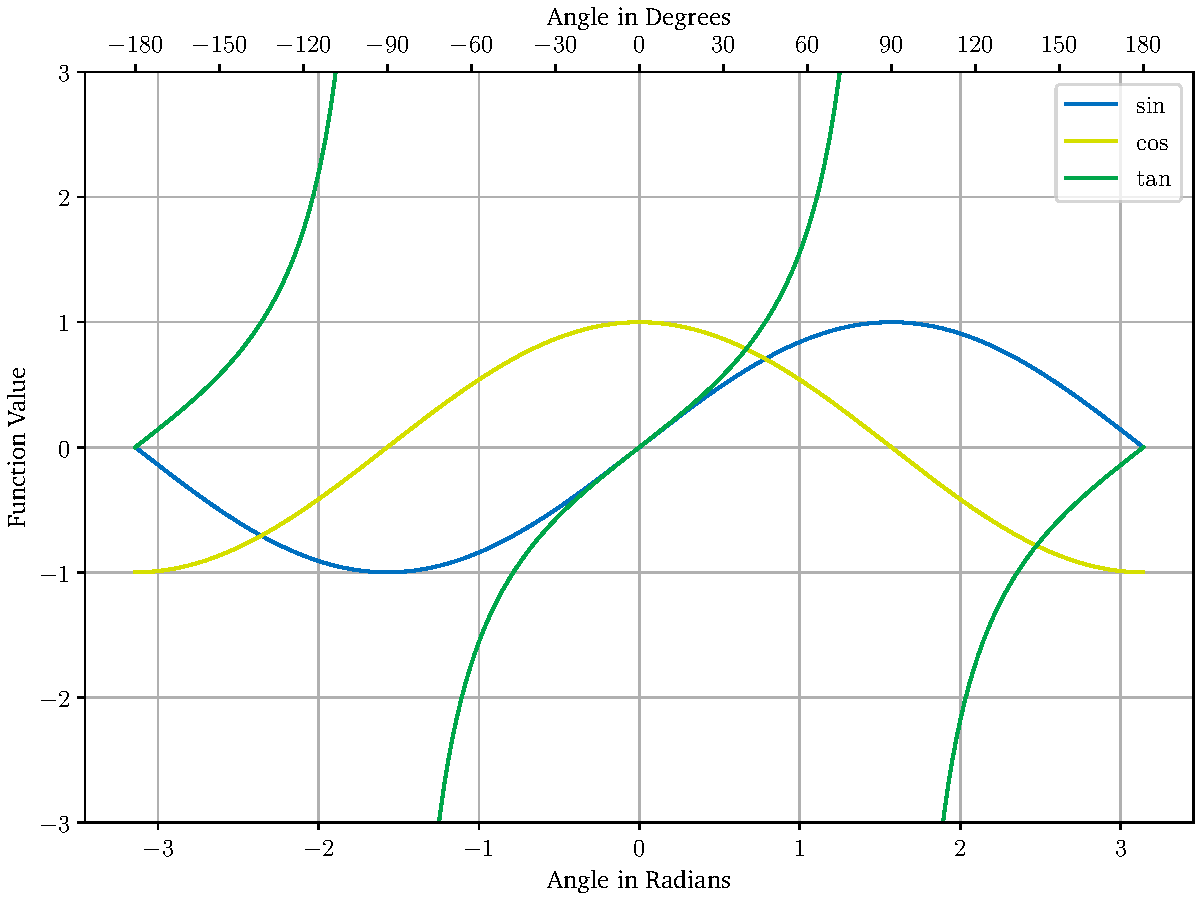
\includegraphics[width=\linewidth]{plots/trigonometric_functions.pdf}
    \caption[Plot comparison of trigonometric functions]{Plot comparison of trigonometric functions}
    \label{fig:trigonometric-func}
\end{figure}

Trigonometric functions are used as relation between apparent power $S$, active $P$ and reactive power $Q$.
While in discription of dynamics, the planning of networks or connection of machines, often the cosinodal function and therefore its value is present in the feeling of (engineering) people.
In stability analysis often the $\tan$ function is used, simply because its directly connecting onle active and reactive power, and because some athematic reformulations are possible with that. 
\autoref{fig:trigonometric-func} is illustrating relations of these functional values to the angle in rad and degree, while \autoref{tab:trigonometric-func} gives a numerical connection.
This shall increase the feeling and evaluation of this thesis readers.

\begin{table}[H]
    \centering
    \small
    \caption{Comparison of trigonometric functions dependent on the angle $\phi$ in degree or radians}
    \label{tab:trigonometric-func}
    \vspace*{12pt}
    \begin{tabularx}{\linewidth}{XXXXX}
        \textbf{Angle in $^\circ$} & \textbf{Angle in rad} & \textbf{$\sin$} & \textbf{$\cos$} & \textbf{$\tan$} \\ \toprule
        0   & 0         & 0         & 1         & 0 \\
        10  & 0.1745    & 0.1736    & 0.9848    & 0.1763 \\
        20  & 0.3490    & 0.3420    & 0.9397    & 0.3640 \\
        30  & 0.5236    & 0.5       & 0.8660    & 0.5774 \\
        40  & 0.6981    & 0.6428    & 0.7660    & 0.8391 \\
        50  & 0.8727    & 0.7660    & 0.6428    & 1.1918 \\ 
        60  & 1.0472    & 0.8660    & 0.5       & 1.7321 \\
        70  & 1.2217    & 0.9397    & 0.3420    & 2.7475 \\
        80  & 1.3962    & 0.9848    & 0.1736    & 5.6713 \\
        90  & 1.5708    & 1         & 0         & $\nexists$ \\
        120 & 2.0944    & 0.8660    & -0.5      & -1.7321 \\
        150 & 2.6180    & 0.5       & -0.8660   & -0.5774 \\
        180 & 3.1416    & 0         & -1        & 0 \\
        \bottomrule
    \end{tabularx}
\end{table}

\section{Description of the Power System Simulation process}
\label{app:power-system-modeling}

In this appendix section, the general process of power system simulation is described. As this thesis is aiming to understand voltage stability and processes in longer periods of time, these explanations apply to pointer-based simulations, called RMS simulations. Meaning that the considered effects are slower electromechanical nature instead of faster electromagnetic ones. The in this thesis used Python framework \glqq \textit{diffpssi}\grqq~is based on this type of simulation, and due to its open-source based nature traceable.

\begin{figure}[H]
    \centering
    % \includegraphics[width=\textwidth]{fundamentals/power-system-simulation-process.pdf}
    \missingfigure{Power system simulation process}
    \caption{Power system simulation process; own illustration}
    \label{fig:power-system-simulation-process}
\end{figure}

\commenting{
    Really basic: (?)
    \begin{itemize}
        \item RMS vs EMT simulation (-> meaning one cannot simulate other faults than 3ph w/o ground)
        \item Phasor description
        \item Basic formulation: Static (algebraic) and dynamic (differential) equations
        \item Using of solvers (Integrators) for time domain simulation
        \item Using of different optimizatinon algorithms for steady state (load flow) simulation -> initial values
    \end{itemize}
    Less basic and more advanced:
    \begin{itemize}
        \item rountines in the framework
        \item two types: Algebraic and Differential equations have to be solved at each time step -> What is which? Which operational equipment is typically described with which type of equation?
        \item per unit system applying for easier simulation (different voltage levels)
        \item ...
    \end{itemize}
}

%%%%%%%%%%%%%%%%%%%%%%%%%%%%%%%%%%%%%%%%%%
% \section{Jacobian based voltage stability criterions}
% \label{app:jacobian-voltage-indices}

% \textcite{danish_2015} is showing, describing, and referencing some voltage stability indices based on the Jacobian matrix. The following table is a collection of these indices.

% \begin{sidewaystable}[H]
%     \centering
%     \small
%     \caption{Jacobian based voltage stability criterions; after \textcite{danish_2015}}
%     \vspace*{12pt}
%     \renewcommand{\arraystretch}{2}
%     \begin{tabularx}{23cm}{llXXl}
%         % \toprule
%         \textbf{Index} & \textbf{Abbreviation} & \textbf{Calculation} & \textbf{Stability Threshold} & \textbf{Reference} \\
%         \toprule
%         Tangent Vector Index & \acs{TVI} & $\mathrm{TVI}_i=\left\lvert \frac{\dd{V_i}}{\dd{\lambda}}\right\rvert^{-1}$ & depending on load increase & \\ \midrule
%         Test Function & & $t_{cc}=\left\lvert e^T_c \cdot \mab{J} \times \mab{J}_{cc}^{-1} \cdot e_c\right\rvert$ & details are given in reference & \\ \midrule
%         Second Order Index & $i$ & $i=\frac{1}{i_0} \cdot \sigma_\mathrm{max} \cdot \big( \dv{\sigma_\mathrm{max}}{\lambda_\mathrm{total}} \big)^{-1}$ & $i > 0$ & \\ \midrule
%         Minimum Eigenvalue & & $\Delta V=\sum_{i} \frac{\xi_i\eta_i}{\lambda_i} \Delta Q$ & all eigenvalues should be positive & \\ \midrule
%         Minimum Singular Value & & $\begin{bmatrix} \Delta \vartheta \\ \Delta V \end{bmatrix}=\mab{V} \sum^-1 \mab{U}^T \begin{bmatrix} \Delta F \\ \Delta G \end{bmatrix}$ & details are given in reference & \\ \midrule
%         Predicting Voltage Collapse & & $\frac{V}{V_0}$ & the smallest index value & \\ \midrule
%         Impedance Ratio & & $\frac{Z_ii}{Z_i}$ & $\frac{Z_ii}{Z_i} \leq 1$ & \\
%         \bottomrule
%     \end{tabularx}
% \end{sidewaystable}



% %%%%%%%%%%%%%%%%%%%%%%%%%%%%%%%%%%%%%%%%%%
% \section{Comparison of System based and Jacobian based indices}
% \label{app:jacobian-vs-system-indices}

% %%%%%%%%%%%%%%%%%%%%%%%%%%%%%%%%%%%%%%%%%%
% %%%%%%%%%%%%%%%%%%%%%%%%%%%%%%%%%%%%%%%%%%
\chapter{Modeling}

%%%%%%%%%%%%%%%%%%%%%%%%%%%%%%%%%%%%%%%%%%
\section{Admittance Calculation of a Two-Port}
\label{app:admittance-deduction}

Follwing part shall just give a short, but complete and clear overview, how the admittance matrix of a two-port system is calculated.
Therefore the main focus of this thesis, a two-port with variable translation ratio, is kept.

%%%%%%%%%%%%%%%%%%%%%%%%%%%%%%%%%%%%%%%%%%
\section{Analytical Calculation of Simple Nose Curves}
\label{app:analytical-nose-curve}

Some blibla and equations about the analytical calculation of simple nose curves.


%%%%%%%%%%%%%%%%%%%%%%%%%%%%%%%%%%%%%%%%%%
\section{Alternative Current Injection Model}
\label{app:current-injection-model}

\textcite{machowski_2020} describes another way of modeling a \acs{OLTC} transformer with variable ratio.
This model is looking at the shunt brnaches as current injections, which are added to the individual busses.
Beneficial, the system admittance matrix is staying symmetrical, while the different transformer state(s) are represented by the different current injections.
This can be mathematically expressed by following set of equations:
\begin{align}
    \begin{bmatrix}
        \underline{I}_1 \\
        -\underline{I}_2
    \end{bmatrix} &=
    \begin{bmatrix}
        \underline{Y}_\mathrm{T} & -\underline{Y}_\mathrm{T} \\
        -\underline{Y}_\mathrm{T} & \underline{Y}_\mathrm{T}
    \end{bmatrix}
    \begin{bmatrix}
        \underline{U}_1 \\
        \underline{U}_2
    \end{bmatrix} -
    \begin{bmatrix}
        \Delta \underline{I}_1 \\
        \Delta \underline{I}_2
    \end{bmatrix}\text{, where } \notag \\[12pt]
    \begin{bmatrix}
        \Delta \underline{I}_1 \\
        \Delta \underline{I}_2
    \end{bmatrix} &=
    \begin{bmatrix}
        \underline{0} & (\underline{\vartheta}-1)\underline{Y}_\mathrm{T} \\
        -(\underline{\vartheta}^*+1)\underline{Y}_\mathrm{T} & (\underline{\vartheta}^*\underline{\vartheta}+1)\underline{Y}_\mathrm{T}
    \end{bmatrix}
    \begin{bmatrix}
        \underline{U}_1 \\
        \underline{U}_2
    \end{bmatrix} \text{ leading to } \notag \\[12pt]
    \underline{\mab{Y}}_\mathrm{\Pi,T,Current~Injection}&= 
    \begin{bmatrix}
        \underline{Y}_\mathrm{T} & -\underline{Y}_\mathrm{T} \\
        -\underline{Y}_\mathrm{T} & \underline{Y}_\mathrm{T}
    \end{bmatrix} -
    \begin{bmatrix}
        \underline{0} & (\underline{\vartheta}-1)\underline{Y}_\mathrm{T} \\
        -(\underline{\vartheta}^*+1)\underline{Y}_\mathrm{T} & (\underline{\vartheta}^*\underline{\vartheta}+1)\underline{Y}_\mathrm{T}
    \end{bmatrix} \notag % \label{eq:admittance-oltc-2}
\end{align}

%%%%%%%%%%%%%%%%%%%%%%%%%%%%%%%%%%%%%%%%%%
\section{Program Structure for the discrete OLTC Control}

\begin{figure}[H]
    \centering
    \missingfigure{Program Plan OLTC}
    \caption[Program or algorithmic structure for the control scheme of the OLTC control]{Program or algorithmic structure for the control scheme of the OLTC control}
    \label{fig:oltc-program-plan}
\end{figure}

%%%%%%%%%%%%%%%%%%%%%%%%%%%%%%%%%%%%%%%%%%
\section{Program Structure for the discrete FSM Control}

\begin{figure}[H]
    \centering
    \missingfigure{Program Plan FSM}
    \caption[Program or algorithmic structure for the control scheme of the FSM control]{Program or algorithmic structure for the control scheme of the FSM control}
    \label{fig:fsm-program-plan}
\end{figure}

%%%%%%%%%%%%%%%%%%%%%%%%%%%%%%%%%%%%%%%%%%
\section{Class Diagrams}

\subsection{Extended Class Diagram of the Transformer Architecture}

\subsection{Extended Class Diagram of the OLTC Transformer}

\subsection{Extended Class Diagram of the Discrete OLTC Control}
\subsection{Extended Class Diagram of the Discrete FSM Control}

\subsection{Class Diagram of the Class Nose Curves}
\label{app:nose-curve}

\begin{figure}[H]
    \centering
    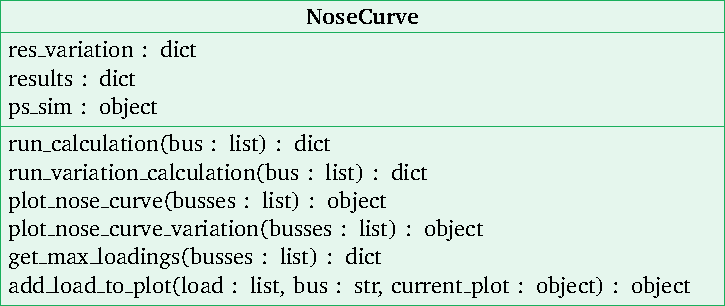
\includegraphics[width=12cm]{tikz_graphics/images/class_diagram_nosecurve_complete.pdf}
    \caption{Complete class diagram of the class Nose Curves; including all attributes and methods with data types, returns, and inputs}
    \label{fig:class-diagram-nose-curves}
\end{figure}


\subsection{Extended Class Diagram of the Class ViolationIntegral}
\subsection{Extended Class Diagram of the Class CriticalTimes}

% %%%%%%%%%%%%%%%%%%%%%%%%%%%%%%%%%%%%%%%%%%
% \section{OLTC control}


%%%%%%%%%%%%%%%%%%%%%%%%%%%%%%%%%%%%%%%%%%
%%%%%%%%%%%%%%%%%%%%%%%%%%%%%%%%%%%%%%%%%%
\chapter{Validation}
\label{app:validation}

%%%%%%%%%%%%%%%%%%%%%%%%%%%%%%%%%%%%%%%%%%
\section{Datails About Used Networks}
\label{app:networks}

\subsection{Single-Machine Infinite Bus-Bar Model}
\label{app:smib-model}

\commenting{Table with parameter details}

\subsection{SMIB Model with Additional Load}
\label{app:smib-w-load}

\commenting{Table with parameter details}


%%%%%%%%%%%%%%%%%%%%%%%%%%%%%%%%%%%%%%%%%%
\section{Additional Plots from the  Pi Model Validation}
\label{app:add-validation-plots}

\begin{figure}[H]
    \centering
    \includegraphics[width=\linewidth]{development_files/validation/data/s_n_comp_complete.pdf}
    \caption[Model results concerning the variation of the rated apparent power]{Voltage results of the $\Pi$-modeled transformer in the \acs{SMIB} model between PowerFactory and the Python framework; Variation of the rated apparent power $S_\mathrm{n}$; Left column is showing the data for the Pathon module \textit{diffpssi}, on the right the comparative tool \textit{DIgSILENT PowerFactory}}
    \label{fig:valid-s-compl}
\end{figure}

\begin{figure}[H]
    \centering
    \includegraphics[width=\linewidth]{development_files/validation/data/s_n_comp_1100mva.pdf}
    \caption{Comparison of one variation parameter between \textit{diffpssi} and \textit{DIgSILENT PowerFactory}; each plot focussing on one bus in the variation of the rated apparent power $S_\mathrm{n}$}
    \label{fig:valid-s-1100}
\end{figure}

\begin{figure}[H]
    \centering
    \includegraphics[width=\linewidth]{development_files/validation/data/theta_comp_complete.pdf}
    \caption{Comparison of the $\Pi$-modeled transformer in the \acs{SMIB} model between PowerFactory and the Python framework}
    \label{fig:valid-ratio-comp}
\end{figure}

\begin{figure}[H]
    \centering
    \includegraphics[width=\linewidth]{development_files/validation/data/theta_comp_ratio09.pdf}
    \caption{Comparison of one variation parameter between \textit{diffpssi} and \textit{DIgSILENT PowerFactory}; each plot focussing on one bus in the variation of the longitudinal transformer ratio $\vartheta$}
    \label{fig:valid-ratio-09}
\end{figure}

%%%%%%%%%%%%%%%%%%%%%%%%%%%%%%%%%%%%%%%%%%
\section{Additional Plots from the Tap Changer Control Schemes}
\label{app:add-validation-tap-changer}

\subsection{OLTC validation}

For simple load:
\begin{figure}[H]
    \centering
    \includegraphics[width=\linewidth]{development_files/validation/data/tds_oltc_simple-load.pdf}
    \caption{\acf{TDS} for standard discrete \acs{OLTC} control scheme applied to the simple load network}
    \label{fig:valid-ratio-09}
\end{figure}

For SMIB with load:
\begin{figure}[H]
    \centering
    \includegraphics[width=\linewidth]{development_files/validation/data/tds_oltc_ex-smib.pdf}
    \caption[Time Domain Result of the OLTC control scheme applied on the extended \acs{SMIB} network]{\acf{TDS} of the standard discrete \acs{OLTC} control scheme; Result of the extended or modified \acs{SMIB} model with additional load}
    \label{fig:tds-oltc-ex-smib}
\end{figure}

\begin{figure}[H]
    \centering
    \includegraphics[width=\linewidth]{development_files/validation/data/oltc_ex-smib_integrator.pdf}
    \caption{Internal signal of the standard discrete \acs{OLTC} control: The integrator signal, representing the time constant for enabling the switching operation}
    \label{fig:int-signal-oltc-ext-smib-integrator}
\end{figure}

\subsection{FSM validation}

For simple load:
\begin{figure}[H]
    \centering
    \includegraphics[width=\linewidth]{development_files/validation/data/signal_vdead_fsm_simple.pdf}
    \caption{Signal evolution for the voltage difference dependent \acs{FSM} control scheme; Plot of the deadband filtered voltage difference $v_\mathrm{dead}$ for the simple load validation case}
    \label{fig:signal-vdead-fsm-simple}
\end{figure}

For SMIB with load:

\begin{figure}[H]
    \centering
    \includegraphics[width=\linewidth]{development_files/validation/data/tds_fsm_vdiff.pdf}
    \caption[\acs{TDS} for a \acs{FSM} control scheme switching based on the voltage difference]{\acs{TDS} for a \acs{FSM} control scheme switching based on the voltage difference}
    \label{fig:tds-fsm-vdiff-ext-smib}
\end{figure}


\begin{figure}[H]
    \centering
    \includegraphics[width=\linewidth]{development_files/validation/data/tds_fsm_preferred.pdf}
    \caption[Differing \acs{TDS} for a \acs{FSM} control scheme preferring the \acs{FSM}]{Differing \acs{TDS} for a \acs{FSM} control scheme preferring the \acs{FSM}}
    \label{fig:tds-fsm-preferred}
\end{figure}

%%%%%%%%%%%%%%%%%%%%%%%%%%%%%%%%%%%%%%%%%%
%%%%%%%%%%%%%%%%%%%%%%%%%%%%%%%%%%%%%%%%%%
\chapter{Case study}
\end{document}
